\chapter{Analytische Geometrie (Vektoren)}
	Der Zweite Teil des Mathe-Abis bezieht sich auf das Rechnen mit Vektoren.
	Unsere Elemente mit denen wir rechnen, sind nun keine Zahlen (diese werden
	Skalare genannt) mehr, sondern Vektoren. Mit ihnen lassen sich dreidimensionale
	Räume leichter darstellen und berechnen\footnote{Tatsächlich gibt es auch mehr
	Dimensionen die man damit berechnen kann, einige Theorien beschäftigen sich
	sogar mit unendlich-dimensionalen Räumen, 3 Dimensionen reichen uns aber ;)}.

	% Section Einleitung Vektoren und Vektoren im Koordinatensystem
	\section{Einleitung Vektoren und Vektoren im Koordinatensystem}
Vektoren lernt man normalerweise erst richtig in der Oberstufe kennen, deswegen möchten wir uns zu Anfang erst einmal damit beschäftigen, was unsere neuen Elemente (also Vektoren) überhaupt sind.\\
Ein Vektor hat immer eine Richtung und eine Länge. Die verschiedenen Zahlen im Vektor geben an, wie weit der Vektor in die jeweiligen Richtungen geht. In der ersten Zeile ist dann die x-Richtung angegeben, in der zweiten die y-Richtung und der letzten Zeile die z-Richtung. Daraus ergeben sich die geforderten Längen und Richtungen. Man benennt sie normalerweise mit kleinen Buchstaben mit einem Pfeil darüber. Ein Vektor sieht dann so aus:
\[\vec{a}=\begin{pmatrix}
 a_1\\
 a_2\\
 a_3
\end{pmatrix}\]
Ein Vektor muss nicht zwingend in einem Koordinatensystem sein, meist wird dies aber der Fall sein. Es ist ähnlich wie die Koordinatensysteme, die wir bereits kennen, nur mit einer weiteren, dritten Dimension. Des weiteren legen wir fest, dass wir den Punkt P(0|0|0) Ursprung nennen, bei dem unser Start für die Vektoren liegt.

% Rechnen mit Vektoren
\subsection{Rechnen mit Vektoren}
Da die Vektoren erst neu dazu kamen, sollten wir zunächst noch einmal kurz auf die Grundrechenarten eingehen und wie diese bei Vektoren angewendet werden.
\subsubsection{Addition}
\todo[color=red]{Kasten für Formel hinzufügen}
\todo[color=red]{Zusammenfassung-Kasten hinzufügen}
\todo[color=red]{Signalwörter-Kasten hinzufügen}
Die Addition von Vektoren ist recht simpel. Wir addieren einfach die einzelnen Zeilen zueinander:
\[\vec{a}+\vec{b}=
\begin{pmatrix}
 a_1\\
 a_2\\
 a_3
\end{pmatrix}+\begin{pmatrix}
 b_1\\
 b_2\\
 b_3
\end{pmatrix}
=
\begin{pmatrix}
 a_1+b_1\\
 a_2+b_2\\
 a_3+b_3
\end{pmatrix} \]
Hier wird vielleicht auch ersichtlich, wie sich die Richtung eines Vektors zusammensetzt, wenn man ihn wie folgt umschreibt:
\[\vec{a}=
\begin{pmatrix}
 a_1\\
 a_2\\
 a_3
\end{pmatrix}=
\begin{pmatrix}
 a_1\\
 0\\
 0
\end{pmatrix} +
\begin{pmatrix}
 0\\
 a_2\\
 0
\end{pmatrix} +
\begin{pmatrix}
 0\\
 0\\
 a_3
\end{pmatrix}
\]
\subsubsection{Subtraktion}
\todo[color=red]{Kasten für Formel hinzufügen}
\todo[color=red]{Zusammenfassung-Kasten hinzufügen}
\todo[color=red]{Signalwörter-Kasten hinzufügen}
Entsprechend kann man auch zwei Vektoren voneinander abziehen. Die Subtraktion erfolgt analog zur Addition. Damit kann man auch den Vektor zwischen zwei Punkten berechnen (Ziel minus Angriff):
\[\vec{a}-\vec{b}=\begin{pmatrix}
 a_1-b_1\\
 a_2-b_2\\
 a_3-b_3
\end{pmatrix}\]
\subsubsection{skalare Faktoren}
\todo[color=red]{Kasten für Formel hinzufügen}
\todo[color=red]{Zusammenfassung-Kasten hinzufügen}
\todo[color=red]{Signalwörter-Kasten hinzufügen}
Mit einem Faktor kann man einen Vektor ums c-Fache vergrößern (oder Verkleinern), bzw. mit einem negativen Faktor die Richtung des Vektors auch um \(180^{\circ}\) drehen. Der Pfeil auf der Linie ist dann einfach auf der anderen Seite. Steht der skalare Faktor vor (oder auch hinter) dem Vektor, so ist das das Gleiche, wie wenn man das Skalar mit jeder Zeile multipliziert:
\[c\cdot \vec{a}=
\begin{pmatrix}
 c\cdot a_1\\
 c\cdot a_2\\
 c\cdot a_3
\end{pmatrix}
\]
\subsubsection{Betrag (Länge) eines Vektors}
\todo[color=red]{Kasten für Formel hinzufügen}
\todo[color=red]{Zusammenfassung-Kasten hinzufügen}
\todo[color=red]{Signalwörter-Kasten hinzufügen}
Will man die Länge eines Vektors ermitteln, so bekommt man ein Skalar mit eben dieser Länge. Man berechnet diesen, indem man den Satz des Pythagoras anwendet, allerdings für 3 Dimensionen. Das sieht dann wie folgt aus:
\[|\vec{a}|=\sqrt{a_1^2+a_2^2+a_3^2}\]
\subsubsection{Skalarprodukt}
\todo[color=red]{Kasten für Formel hinzufügen}
\todo[color=red]{Zusammenfassung-Kasten hinzufügen}
\todo[color=red]{Signalwörter-Kasten hinzufügen}
Eine Art des Produkts bei Vektoren ist das Skalarprodukt. Man multipliziert hier die Länge des Vektors, auf den anderen projektiert, mit der kompletten Länge des anderen Vektors. Wie man sich das genauer vorstellen kann, findet man im Internet oder hier in unserem Kurs ;). Man berechnet das Skalarprodukt wie folgt:
\[\vec{a}\cdot \vec{b}=a_1\cdot b_1+a_2\cdot b_2+a_3\cdot b_3\]
Somit haben wir aus zwei Vektoren ein Skalar (eine Zahl) gemacht. Welche Bedeutung dies hat sehen wir, wenn wir uns die Definition genauer anschauen. Mathematisch sieht diese wie folgt aus:
\[\vec{a}\cdot \vec{b}=|\vec{a}|\cdot |\vec{b}|\cdot cos(\varphi)\]
Mit dieser Relation kann man die Projektion erkennen und sieht auch, dass zwei orthogonale Vektoren das Skalarprodukt 0 haben. Mit dieser kann man jedoch auch den Winkel zwischen zwei Vektoren berechnen. Zwar ist dies recht leicht umzustellen, da dies aber eine wichtige Relation ist, werden wir sie noch einmal umgestellt aufschreiben\footnote{Beachtet bitte, dass es immer 2 Winkel gibt. Beide zusammen ergeben \(180^{\circ}\). Man gibt aber immer den kleineren Winkel an. Bekommt ihr also einen Winkel der größer ist als \(90^{\circ}\), so ist euer richtiger Winkel einfach: \(\alpha=180^{\circ}-\beta\)}:
\[cos(\varphi)=\frac{ | \vec{a}\cdot \vec{b} | }{|\vec{a}|\cdot |\vec{b}|}\]
\subsubsection{Kreuzprodukt}
\todo[color=red]{Kasten für Formel hinzufügen}
\todo[color=red]{Zusammenfassung-Kasten hinzufügen}
\todo[color=red]{Signalwörter-Kasten hinzufügen}
Das Kreuzprodukt ist in den meisten Klassen kein Unterrichtsstoff und wird auch nicht in der Prüfung abgefragt. Trotzdem wollen wir es hier ansprechen, da dies eine einfache Art ist, einen Normalenvektor (später bei den Ebenen) zu bestimmen und bei der Prüfung darf dieser auch verwendet werden. Das Kreuzprodukt ergibt nämlich immer einen Vektor, der zu den zwei anderen rechtwinklig steht, was der Definition eines Normalenvektors entspricht.\\
Ihn aufzustellen, mag bei den ersten Versuchen ein wenig kompliziert erscheinen. Das zu üben lohnt sich jedoch erheblich. In die erste Zeile des Kreuzprodukts (welcher ein Vektor ist) schreibt man \(a_2\cdot b_3-a_3\cdot b_2\). Nun schreibt man in den weiteren Zeilen jeweils den Buchstaben ab und addiert immer 1 auf die Indizes (aus einer 3 wird dann eine 1!):
\[\vec{a} \times \vec{b}=
\begin{pmatrix}
 a_2b_3-a_3b_2\\
 a_3b_1-a_1b_3\\
 a_1b_2-a_2b_1
\end{pmatrix}\]
Es gibt auch noch eine weitere Methode, die wir hier aber nicht schriftlich festhalten wollen. Diese besprechen wir dann im Kurs selbst.

\subsubsection{Lineare Abhängigkeit}
\todo[color=red]{Kasten für Formel hinzufügen}
\todo[color=red]{Zusammenfassung-Kasten hinzufügen}
\todo[color=red]{Signalwörter-Kasten hinzufügen}
Für das Abitur braucht ihr die Definition der linearen Abhängigkeit nicht mehr komplett zu kennen. Jedoch solltet ihr die Frage, ob zwei Vektoren linear abhängig sind, beantworten können (die Definition befasst sich auch mit mehreren Vektoren). Entscheidend wird dies, wenn wir Geraden oder Ebenen vergleichen wollen. Können wir einen Vektor durch einen anderen mit einem konstanten Faktor k multipliziert darstellen, sind diese linear abhängig. Bei 
\(k\cdot \begin{pmatrix}
 1\\
 -2\\
 4
\end{pmatrix}=\begin{pmatrix}
 -4\\
 8\\
 8
\end{pmatrix}\)
zum Beispiel überlegt man zunächst, wie man von 1 auf -4 kommt. Das gilt wenn k=-4 ist. Überprüft man das nun, so stimmt mit diesem k auch die zweite Zeile. Die dritte Zeile macht uns dann aber einen Strich durch die Rechnung, so dass diese Vektoren linear unabhängig sind (wäre die letzte Zeile -16 so würde es passen). Linear abhängig sind zwei Vektoren, wenn sich ein k finden lässt, sodass gilt:
\[\vec{a}=k\cdot \vec{b}\]



	% Section Geraden
	\section{Geraden}
Geraden können wir mithilfe von Vektoren im Raum darstellen. Schauen wir uns zunächst noch einmal an, wie wir das in der Analysis gemacht haben, um die Parallelen aufzuzeigen: f(x)=mx+c. Mit Vektoren stellt man dies ganz ähnlich dar. Zuerst hat man einen Stützvektor, der dem c ähnlich ist und ohne Variable in der Funktion steht. Der Richtungsvektor gibt, wie schon der Name sagt, die Richtung an. Vor ihm steht eine skalare Variable (meist s oder t genannt) welche sich mit unserem x vergleichen lässt. Der Richtungsvektor entspricht also der Steigung m (diese gibt ja ebenfalls die Richtung an). Somit können wir jeden Punkt \(\vec{x}\) (als Ortsvektor dargestellt) der auf unserer Geraden ist, angeben (\(\vec{a}\) ist der Stützvektor, \(\vec{b}\) der Richtungsvektor):
\[g:\ \vec{x}=\vec{a}+s\cdot \vec{b}\]
 

	% Section Ebenen
	\section{Ebenen}
Ebenso wie Geraden, können wir im 3D-Raum auch Ebenen darstellen. Dafür gibt es drei verschiedene Möglichkeiten die wir verwenden.

\subsection{Parameterform}
Um eine Ebene anhand von drei Punkten aufzustellen, ist die Parameterform am einfachsten. Sie ähnelt der Geradengleichung (ist also übersichtlicher auf dem ersten Blick) und die anderen beiden Formen lassen sich daraus leicht aufstellen (mit denen leichter weiter zu rechnen ist). Deshalb werden wir diese Form als Erstes zeigen, auch wenn man sie seltener nutzt. Zuerst haben wir wieder einen Stützvektor, wie bei der Geraden. Jedoch haben wir statt einem gleich zwei 'Richtungsvektoren', die Spannvektoren genannt werden (sie Spannen die Ebene auf). Diese berechnet man, indem man zwei Vektoren zwischen je zwei Punkten berechnet und eine skalare Variable mit ihnen multipliziert:
\[E:\ \vec{x}=\vec{a}+s\cdot \vec{b}+t\cdot \vec{c}\]

\subsection{Normalenform}
Mit der Normalenform können wir leichter rechnen, vergleichen und Abstände bestimmen. Die Überlegung dahinter ist ein wenig umständlicher, bei näherer Betrachtung aber nicht zwingend schwerer. Zuerst müssen wir den Normalenvektor \(\vec{n}\) finden, welcher orthogonal auf der Ebene steht. Am einfachsten und schnellsten geht das, indem wir das Kreuzprodukt der Spannvektoren berechnen, wodurch wir direkt den Normalenvektor erhalten. Eine umständlichere Variante wäre, das Skalarprodukt der Spannvektoren mit dem Normalenvektor 0 zu setzen (aufgrund der Orthogonalität) und das lineare Gleichungssystem zu lösen.\\
Nur wie kombinieren wir jetzt die Vektoren? Die Überlegung ist folgende: Wir ziehen von einem Punkt auf der Ebene den wir kennen (der Stützvektor \(\vec{a}\)), den Punkt den wir überprüfen wollen (\(\vec{x}\)) ab und bekommen so einen Vektor, von einem Punkt zum anderen. Liegt dieser auch auf der Ebene, so ist dieser rechtwinklig zum Normalenvektor (der ja zu jedem Vektor auf der Ebene orthogonal ist). Ist das nicht der Fall, liegt der Punkt irgendwie anders im Raum, aber nicht auf der Ebene. Das heißt, wenn wir den neu berechneten Vektor mit dem Normalenvektor skalar multiplizieren und der Punkt liegt auf der Ebene, so ist das Ergebnis 0:
\[E:\ (\vec{a}-\vec{x})\cdot\vec{n}=0\]
Wichtig hier zu erwähnen ist auch die hessesche Normalform. Diese unterscheidet sich lediglich durch den normierten Normalenvektor (dargestellt als \(\hat n\)). Normiert heißt hier, dass wir ihn durch die Länge teilen, er also nur noch die Länge 1 hat. Somit sieht die Hess'sche Normalenform um den Abstand d zu einem Punkt zu ermitteln, wie folgt aus:
\[E:\ (\vec{a}-\vec{x})\cdot \frac{1}{|\vec{n}|}\vec{n}=(\vec{a}-\vec{x})\cdot \hat{n}=d\]

\subsection{Koordinatenform}
An der Koordinatenform gibt es nicht viel zu verstehen. Wir müssen nur lernen, sie aufzustellen. Letztendlich ist sie aber eine Umformung der Normalenform. Hierzu brauchen wir zuerst den Normalenvektor, welchen wir mit dem erst einmal unbekannten Vektor \(\vec{x}\) skalar multiplizieren\footnote{Einfacher gesagt, setzt einfach die entsprechende Zeile des Normalenvektors zu der entsprechenden x-Zeile ein, usw.}. Auf der rechten Seite der Gleichung steht dann die Zahl w, die raus kommt, wenn wir das Skalarprodukt einmal ausrechnen, indem wir den Stützvektor \(\vec{a}\) für \(\vec{x}\) einsetzen:
\[n_1x_1+n_2x_2+n_3x_3=w \mathrm{\ (anders\ geschrieben\ } \vec{n}\cdot \vec{x}=w)\]
Analog zur Hesseschen Normalform ist es auch möglich, die Koordinatenform anzugeben, indem man zuerst w abzieht und dann den gesamten Term durch die Länge des Normalenvektors teilt. So bekommt man den Abstand d der Ebene zum Punkt \(\vec{x}\):
\[\frac{n_1x_1+n_2x_2+n_3x_3-w}{|\vec{n}|}=d\]


	% Section Darstellung im Dreidimensionalen
	\section{Darstellung im Dreidimensionalen}
	\todo[color=red]{Kasten für Formel hinzufügen}
	\todo[color=red]{Zusammenfassung-Kasten hinzufügen}
	\todo[color=red]{Signalwörter-Kasten hinzufügen}
	Sollen Punkte, Ebenen oder Geraden in ein Koordinatensystem gezeichnet werden,
	so sollten wir uns zunächst noch einmal Gedanken darüber machen, wie man die
	Achsen einträgt. Die y-Achse wird nach rechts hin aufgetragen, die z-Achse nach
	oben hin. Bei der x-Achse, welche nach links vorne gezeichnet wird
	(\(45^{\circ}\) zur y-Achse), besteht die Besonderheit, dass eine Längeneinheit
	nur halb so lang gezeichnet wird. Das ist auch bei der Einteilung der x-Achse
	zu beachten!

	\subsection{Gerade}
		\todo[color=red]{Kasten für Formel hinzufügen}
		\todo[color=red]{Zusammenfassung-Kasten hinzufügen}
		\todo[color=red]{Signalwörter-Kasten hinzufügen}
		Auch wenn es selten vorkommt, werden wir zur Sicherheit erwähnen, wie man sie
		einzeichnet. Nehmt dazu den Stützvektor und zeichnet ihn ein. Ebenso wie einen
		zweiten Vektor auf der Gerade (den bekommt ihr, indem ihr zum Beispiel s=1
		setzt). Dann verbindet ihr die Punkte mit einer Linie und schon habt ihr die
		Gerade.

	\subsection{Ebenen (Spurpunkte \& -geraden)}
		\todo[color=red]{Kasten für Formel hinzufügen}
		\todo[color=red]{Zusammenfassung-Kasten hinzufügen}
		\todo[color=red]{Signalwörter-Kasten hinzufügen}

    	\begin{figure}[h]
    		\centering
    		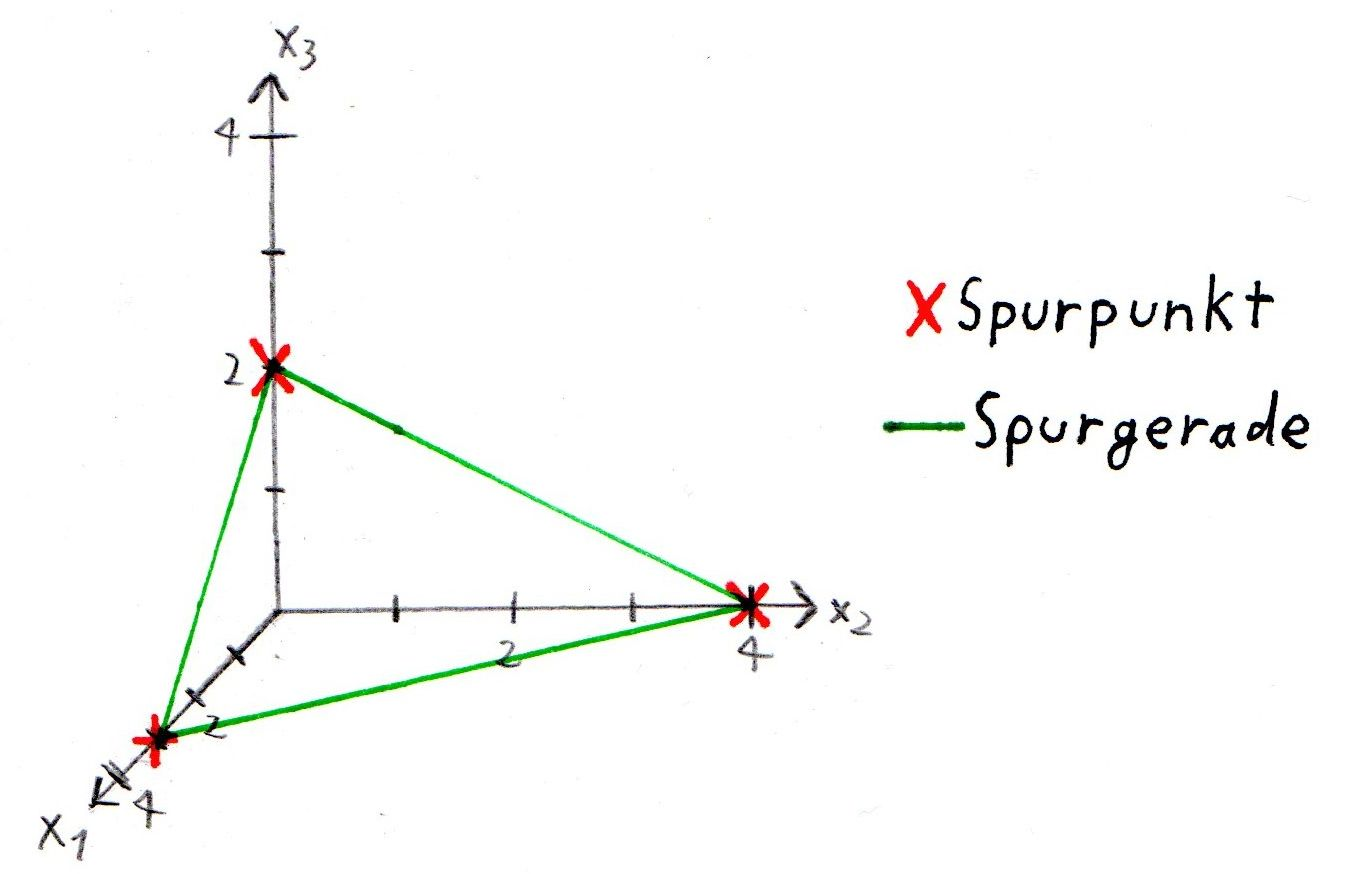
\includegraphics[scale=0.2]{Images/Spurpunkte.jpeg}
    		\caption{Spurpunkte und Geraden einer Ebene}
    	\end{figure}

		Um Ebenen darzustellen, nimmt man sich Spurpunkte bzw. -geraden zur Hilfe.
		Wenn nicht anders verlangt, raten wir zu den Spurpunkten. Das sind die Punkte,
		in denen die Ebene die Achsen schneidet. Man berechnet sie einfach, indem man
		(für das Schneiden mit der x-Achse) y=z=0 setzt und erhält so einen Wert für
		x. Mit den anderen Punkten, die man natürlich synchron dazu berechnet, spannt
		sich dann eine Ebene auf.\\
		Die Spurgeraden sind Geraden, die durch jeweils zwei Spurpunkte gehen. Diese
		benötigt man lediglich bei Ebenen, die in der Parameterform dargestellt sind.
		Dazu setzt man bei \(\vec{x}\) einfach eine Koordinate 0 und berechnet dann
		die Parameter in dieser Zeile.

	\subsection{einfache geometrische Formen im Raum}
		\todo[color=red]{Kasten für Formel hinzufügen}
		\todo[color=red]{Zusammenfassung-Kasten hinzufügen}
		\todo[color=red]{Signalwörter-Kasten hinzufügen}
		Jegliche Formen im Raum darzustellen, ist recht leicht. Hierzu setzt ihr
		einfach alle angegebenen Punkte ins Koordinatensystem ein und verbindet die
		Punkte (überlegt euch, welche Punkte überhaupt verbunden werden müssen, bei
		einem Quadrat ABCD ist es nicht sinnvoll, AC und BD zu verbinden).


	% Section Lagebeziehungen
	\section{Lagebeziehungen}
	\todo[color=purple]{Kasten für Formel hinzufügen}
	\todo[inline,color=red]{Zusammenfassung-Kasten hinzufügen}
	\todo[inline,color=red]{Signalwörter-Kasten hinzufügen}
	Zuletzt wollen wir noch die unterschiedlichen Lagebeziehungen besprechen.
	Manchmal wird explizit nach ihnen gefragt, manchmal brauchen wir sie aber auch,
	um im Wahlteil Anwendungsaufgaben beantworten zu können\footnote{wir werden
	hier nicht explizit auf die Erklärungen für Anwendungsaufgaben eingehen. Zum
	einen, weil es aus typografischen Gründen keinen Sinn macht und wir euch zum
	anderen nicht dadurch verwirren wollen. Im Kurs werden wir aber darauf
	eingehen.}. Die hier genannten Verfahren sind nicht die Einzigen, denn nicht
	nur ein Weg führt zur Lösung. Die hier besprochenen Wege sind unserer Meinung
	nach die Einfachsten. Wenn ihr mit eurer eigenen Methode aber besser zurecht
	kommt, ist es weniger sinnig, ausgerechnet unsere zu benutzen. Im Kurs werden
	wir bei Bedarf auch auf andere Wege eingehen.

	% Punkt - Punkt
	\subsection{Punkt - Punkt}
	\todo[color=purple]{Kasten für Formel hinzufügen}
	\todo[color=purple]{Zusammenfassung-Kasten hinzufügen}
	\todo[color=purple]{Signalwörter-Kasten hinzufügen}
	Diese Beziehung dürfte klar sein. Entweder haben wir den gleichen Punkt im Raum
	(was sofort erkennbar wäre) oder aber sie liegen örtlich auseinander. Dann kann
	man angeben, wie weit die Punkte entfernt sind, indem man einen Punkt vom
	anderen abzieht (Ziel minus Angriff) und von diesem neuen Vektor den Betrag
	berechnet, um zu berechnen, um den Abstand zu bestimmen.


	% Punkt - Gerade
	\subsection{Punkt - Gerade}
Hier wollen wir den kleinsten Abstand von der Geraden zum Punkt berechnen\footnote{tatsächlich gibt es ja unendlich viele Abstände, entscheidend ist aber in der Mathematik immer der Kürzeste.}.\\
Zunächst setzt ihr den Punkt in die Gerade ein, um zu überprüfen, ob dieser nicht sogar darauf liegt. Liegt er nicht dort, so müsst ihr zuerst eine Hilfsebene aufstellen. Der Richtungsvektor der Geraden entspricht dann dem Normalenvektor der Hilfsebene. Euer Punkt, der nicht auf der Geraden liegt, ist der Stützvektor der Ebene (somit stellt ihr sicher, dass ein rechter Winkel zwischen Gerade und der Strecke zum Punkt ist). Nun müsst ihr ermitteln, in welchem Punkt die Gerade die Hilfsebene durchstößt. Ab hier ist es lediglich eine \textbf{Punkt - Punkt} - Beziehung die ihr berechnen müsst.\\
Das ganze ist natürlich recht aufwändig und nimmt viel Zeit in Anspruch. Glücklicherweise gibt es aber eine einfachere Variante. Sie mag nicht so ersichtlich sein, auf den ersten Blick. Letztendlich müsst ihr aber lediglich die Formel auswendig lernen. Auf den Beweis und den Gedanken dahinter, werden wir im Kurs näher eingehen. Wir setzen dort dann den angegebenen Punkt \(\vec{x}\) ein, so wie den Stützvektor \(\vec{a}\) und den Richtungsvektor \(\vec{b}\) und bekommen den Abstand d (ist d=0, so liegt der Punkt natürlich auf der Geraden)\footnote{Vor allem durch das Kreuzprodukt scheint das ganze recht komplex auszusehen. Letztendlich ist aber auch das schnell eingeübt.}:
\[d=\frac{|(\vec{a}-\vec{x})\times \vec{b}|}{|\vec{b}|}\]


	% Punkt - Ebene
	\subsection{Punkt - Ebene}
	\todo[color=green]{Kasten für Formel hinzufügen}
	\todo[inline,color=red]{Zusammenfassung-Kasten hinzufügen}
	\todo[inline,color=red]{Signalwörter-Kasten hinzufügen}
	Den Abstand zwischen einem Punkt und einer Ebene berechnet man mit der
	Hesseschen Normalform / Koordinatenform. Ihr müsst für \(\vec{x}\) einfach den
	angegebenen Punkt (dessen Abstand ihr zur Ebene ermitteln wollt) einsetzen und
	habt sofort den Abstand. Zur Wiederholung:
	\formel{\[d=(\vec{a}-\vec{x})\cdot \hat{n} \mathrm{\ bzw\ }
	d=\frac{n_1x_1+n_2x_2+n_3x_3-w}{|\vec{n}|}\]}
	Ist der Abstand 0, so liegt der Punkt natürlich auf der Ebene.


	% Gerade - Gerade
	\subsection{Gerade - Gerade}
\todo[color=red]{Kasten für Formel hinzufügen}
\todo[color=red]{Zusammenfassung-Kasten hinzufügen}
\todo[color=red]{Signalwörter-Kasten hinzufügen}
Beim Betrachten der Lage zwischen zwei Geraden gibt es vier unterschiedliche Möglichkeiten, die wir prüfen müssen. Wir empfehlen euch, zuerst die Richtungsvektoren zu betrachten und dann zu prüfen, ob diese linear abhängig sind oder nicht.\\
\(\star\) Ist dies der Fall, so können sie entweder parallel sein oder liegen sogar aufeinander. Um das herauszufinden, ermittelt ihr einfach den Abstand von einer Geraden zu dem Stützpunkt der anderen Geraden (Beziehung \textbf{Punkt - Gerade}). Ist der Abstand 0, so sind die Geraden identisch, ansonsten sind sie parallel und haben den Abstand d.\\
\(\star\) Sind die Richtungsvektoren nicht linear abhängig, so sind sie windschief oder schneiden sich an einem Punkt. Hierzu setzt man zuerst beide Geraden gleich und löst das LGS. Geht es auf, so schneiden sie sich in diesem Punkt (setzt das s oder t bitte in die entsprechende Gerade ein, um zu schauen an welchen Punkt sie sich schneiden und gebt diesen an).\\
Schneiden sich die beiden Geraden nicht, so sind sie windschief. Dann ist wieder der kürzeste Abstand zwischen den Geraden anzugeben. Hier müsst ihr wieder eine Hilfsebene aufstellen. Diesmal sind die Richtungsvektoren der beiden Geraden die Spannvektoren der Hilfsebene (siehe \textbf{Parameterform}). Aus ihnen könnt ihr sofort die Normalen- oder Koordinatenform mit dem Normalenvektor angeben. Euer Punkt auf der Ebene ist dann einer der Stützvektoren. Der Abstand der Ebene zum Stützvektor (Beziehung \textbf{Punkt - Ebene}) der anderen Geraden ist dann der kleinste Abstand zwischen den windschiefen Geraden.


	% Gerade - Ebene
	\subsection{Gerade - Ebene}
	\todo[color=red]{Kasten für Formel hinzufügen}
	\todo[color=red]{Zusammenfassung-Kasten hinzufügen}
	\todo[color=red]{Signalwörter-Kasten hinzufügen}
	Bei dieser Beziehung gibt es 3 Möglichkeiten, die vorkommen können. Um
	herauszufinden, welche vorliegt, ist zu empfehlen, zunächst Richtungsvektor und
	Normalenvektor zu vergleichen. Man skalar multipliziert einfach diese beiden
	Vektoren und betrachtet das Ergebnis.\\

	\(\star\) Ist das Skalarprodukt 0, so sind die Vektoren orthogonal, sowie
	Gerade und Ebene parallel. Nun berechnet man den Abstand des Stützvektors der
	Gerade zur Ebene (Beziehung \textbf{Punkt - Ebene}). Ist der Abstand 0, so
	liegt die Gerade auf der Ebene, ansonsten kennen wir dessen Abstand d.\\

	\(\star\) Ist das Skalarprodukt nicht 0, so wird die Gerade die Ebene
	durchstoßen. Diesen Punkt kann man herausfinden, indem man in der
	Ebenengleichung \(\vec{x}\) durch die Geradengleichung ersetzt und das LGS
	löst.
	\emph{Vorsicht gilt bei der Winkelbestimmung!} Hier gilt nämlich im Gegensatz
	zu den anderen Lagebeziehungen folgende Formel ( \(\vec{n}\) ist der
	Normalenvektor, \(\vec{a}\) der Richtungsvektor):
	\[cos(\alpha)=\frac{|\vec{n}\cdot \vec{a}|}{|\vec{n}|\cdot |\vec{a}|}\]


	% Ebene - Ebene
	\subsection{Ebene - Ebene}
	\todo[color=red]{Kasten für Formel hinzufügen}
	\todo[color=red]{Zusammenfassung-Kasten hinzufügen}
	\todo[color=red]{Signalwörter-Kasten hinzufügen}
	Auch hier gibt es potentiell 3 Möglichkeiten. Zunächst vergleichen wir die
	Normalenvektoren und schauen, ob diese linear abhängig sind.\\

	\(\star\) Sind sie es, so sind die Ebenen natürlich parallel zueinander. Hier
	wird dann der Abstand von einem Stützvektor der Ebenen zur anderen Ebene
	berechnet (Beziehung \textbf{Punkt - Ebene}). Ist dieser Abstand 0, so sind die
	beiden Ebenen identisch. Ist der Abstand nicht 0, so haben wir 2 parallele
	Ebenen mit dem Abstand d zueinander.\\

	\(\star\) Sind die Normalen nicht linear abhängig, so haben wir die dritte
	Möglichkeit. Die Ebenen schneiden sich. Um die Schnittgerade zu ermitteln,
	setzt man die Ebenen gleich und erhält ein LGS, welches man (mit einer
	Variablen, welche unser 's' ist) löst.
